\documentclass[11pt, oneside]{article}
\usepackage[letterpaper, margin=2cm]{geometry}
\usepackage{MATH566}
%\usepackage{sagetex}

\begin{document}
\noindent \textbf{\Large{Caleb Logemann \\
MATH 566 Discrete Optimization\\
Homework 4
}}

%\lstinputlisting[language=Sage]{03_2.sage}
\begin{enumerate}
  \item % #1 Done
    Write a program that will solve an instance of linear programming by
    enumerating basic feasible solutions and keeping the best one.
    Input to the program is matrix, $A \in \RR^{m \times n}$ and vectors
    $\v{b} \in \RR^m$ and $\v{c} \in \RR^n$

    The following script implements this function that solves a linear
    program by trying all basic feasible solutions.
    The function acheives the same values of the objective function as Sage's
    built in linear program solver.
    \lstinputlisting[language=Sage]{04_1.sage}
    This is the output of the script.
    \begin{verbatim}
        
    \end{verbatim}

  \item % #2 Done
    Convert the following program to equational form and solve it using the
    simplex method.
    \[
      (P) 
      \begin{cases} 
        \begin{array}{lrccccc} 
          \text{maximize}    &x_1  &+  &2x_2 &     &   \\
          \text{subject to}  &x_1  &   &     &\leq & 4 \\
                             &x_1  &+  &x_2  &\leq & 5 \\
                             &-x_1 &+  &x_2  &\leq & 1 \\
        \end{array}\\
        \text{ \hskip 8em } x_1,x_2 \geq 0
      \end{cases}
    \]
    Use Bland's rule for selecting pivots.
    That is, pivot on variable with lowest possible index.
    Use the last tableau to argue that the solution is indeed optimal.
    Plot the set of feasible solutions of (P) and mark the solutions obtained
    after each iteration of the simplex method.

    The new linear program in equational form with slack variables is
    \[
      (P)
      \begin{cases}
        \begin{array}{lr*{11}c}
          \max*        & x_1  &+ &2x_2  &  &    &  &     &  &    &    &  & \\
          \text{s.t.} & x_1  &  &      &+ &x_3 &  &     &  &    &=   &4 & \\
                      & x_1  &+ &x_2   &  &    &+ &x_4  &  &    &=   &5 & \\
                      & -x_1 &+ &x_2   &  &    &  &     &+ &x_5 &=   &1 & \\
                      &      &  &      &  &    &  &     &  &x_i &\ge &0 &1 \le i \le 5 \\
        \end{array}
      \end{cases}
    \]

    An initial basic feasible solution with $x_3 = 4$, $x_4 = 5$ and $x_5 = 1$.
    \begin{align*}
      x_3 &= 4 - x_1 \\
      x_4 &= 5 - x_1 - x_2 \\
      x_5 &= 1 + x_1 - x_2 \\
      z   &= 0 + x_1 + 2x_2
    \end{align*}
    Increasing $x_1$ by 4 results in the following.
    \begin{align*}
      x_1 &= 4 - x_3 \\
      x_4 &= 1 - x_2 + x_3 \\
      x_5 &= 5 - x_2 - x_3 \\
      z   &= 4 + 2x_2 - x_3
    \end{align*}
    Now $x_2$ can be increased by 1.
    \begin{align*}
      x_1 &= 4 - x_3 \\
      x_2 &= 1 + x_3 - x_4 \\
      x_5 &= 4 - 2x_3 - x_4  \\
      z   &= 6 + x_3 - 2x_4 \\
    \end{align*}
    Lastly $x_3$ can be increased by 2.
    \begin{align*}
      x_1 &= 2 + (1/2)x_4 + x_5 \\
      x_2 &= 3 -(3/2)x_4 - x_5 \\
      x_3 &= 2 -(1/2)x_4 - x_5 \\
      z   &= 8 - (5/2)x_4 - x_5 \\
    \end{align*}
    This is the optimal solution because all the coefficients of the objective
    function are negative.

    \begin{center}
        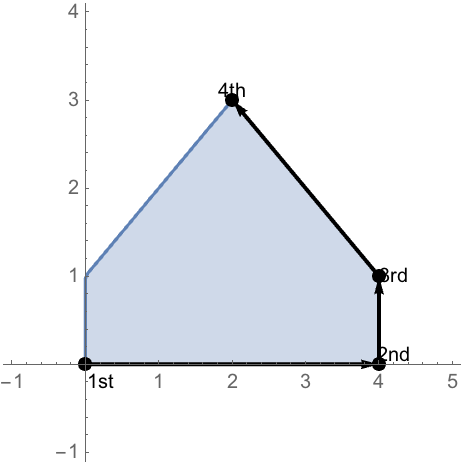
\includegraphics[scale=.5]{Figures/04_1.png}
    \end{center}

  \item % #3 Done
    Use simplex method on the following program:
    \[
      (P) 
      \begin{cases} 
        \begin{array}{lrccccc} 
          \text{maximize}   &x_1  &  &    &     &   \\
          \text{subject to} &x_1  &- &x_2 &\leq &1 \\
                            &-x_1 &+ &x_2 &\leq &2 \\
        \end{array}\\
        \text{ \hskip 8em } x_1,x_2 \geq 0
      \end{cases}
    \]
    What is happening in the computation?

    The new linear program with slack variables is
    \[
      (P) 
      \begin{cases} 
        \begin{array}{lr*{10}c} 
          \text{maximize}   &x_1  &  &    &  &    &  &    &    & \\
          \text{subject to} &x_1  &- &x_2 &+ &x_3 &  &    &=   &1 \\
                            &-x_1 &+ &x_2 &  &    &+ &x_4 &=   &2 \\
                            &     &  &    &  &    &  &x_i &\ge &0 \\
        \end{array}\\
      \end{cases}
    \]

    The initial basic feasible is $x_3 = 1$ and $x_4 = 2$.
    \begin{align*}
      x_3 &= 1 - x_1 + x_2 \\
      x_4 &= 2 + x_1 - x_2 \\
      z   &= 0 + x_1
    \end{align*}
    First increase $x_1$ by 1.
    \begin{align*}
      x_1 &= 1 + x_2 - x_3 \\
      x_4 &= 3 - x_3 \\
      z   &= 1 + x_2 - x_3
    \end{align*}
    Now we see that $x_2$ should be increased however there is no condition
    limiting the increase of $x_2$.
    This implies that the feasible region is unbounded and the objective
    function can be increased indefinitely.

    As can be seen in the following image the feasible region continues
    out to infinity to the right.
    \begin{center}
      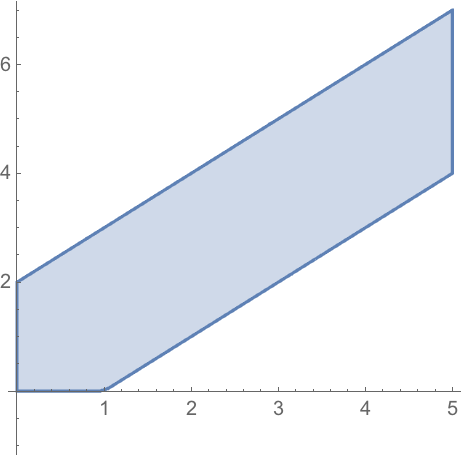
\includegraphics[scale=.5]{Figures/04_2.png}
    \end{center}

  \item % #4
    How would you solve a program 
    $(P)  = \text{maximize } \mathbf{c}^T\mathbf{x} \text{ s.t. } A\mathbf{x} \leq \mathbf{b}, \mathbf{x} \geq \mathbf{0}$
    using the ellipsoid method with an $\varepsilon > 0$ error?
    (Suppose both $(P)$ and its dual $(D)$ are superconsistent.)
    %\emph{(Hint: How to formulate the linear program as finding a point in a polytope? 
    %Use dual program and $\varepsilon$ to guarantee full dimension.)}
\end{enumerate}
\end{document}
